\section{Hardware}

\begin{frame}
	\frametitle{Hardware latencies}
	The hardware itself can be the source of latencies:
	\begin{itemize}
		\item Power-management features uses sleep states that introduce latencies
		\item Throughput features introduce lots of cache levels that are hard to predict
		\item Even CPU features like branch-prediction introduce latencies
		\item Hardware latencies are nowadays unavoidable, but some can be mitigated
		\item It's important to benchmark the hardware platform early during development
	\end{itemize}
\end{frame}

\begin{frame}
	\frametitle{Non-Maskable Interrupts}
	Non-Maskable Interrupts can't be disabled, and can be transparent to the OS
	\begin{itemize}
		\item Common NMIs are System Management Interrupts (SMIs)
		\item SMIs run in a dedicated context, the System Management Mode
		\item It often runs low-level firmware code, like BIOS and EFI
		\item Used for thermal management, remote configuration, and are very opaque
		\item Can't be prevented, predicted, monitored or controlled
		\item Modern CPUs can expose a NMI counter
		\item Kernel-processed NMIs can be instrumented with \code{ftrace}
		\item \code{hwlatdetect} can help measure the NMIs on a given system
	\end{itemize}
	% SMM, SMI
	% hwlatdet
\end{frame}

\begin{frame}
	\frametitle{Deep Firmwares}
	On modern hardware, several firmwares can run outside the control of the Kernel
	\begin{itemize}
		\item The ARM TrustZone can run firmware like OP-TEE, to handle sensitive tasks
		\item Low-level firmware calls can be made by drivers through SMC calls or similar
		\item These firmwares can disable interrupts while they run
		\item Depending on the SoC, we might or might not have control over these firmwares
		\item \code{hwlatdetect} and careful driver analysis can help identify these issues
	\end{itemize}
	% Bios/efi, SMC calls
\end{frame}

\begin{frame}
	\frametitle{Memory access}
	Accessing a virtual address can trigger a Page Fault if:
	\begin{itemize}
		\item The page isn't mapped yet
		\item The address is invalid
	\end{itemize}
	Programs should first access all pages to populate the page-table, then
	pin them with \code{mlockall()}

	On a smaller scale, caching can also impact memory access time, and be affected by
	processes running on other CPUs
\end{frame}

\begin{frame}
	\frametitle{Hyperthreading}
	Some CPU cores have 2 pipelines feeding the same ALU. This is known as \textbf{Hyperthreading}
	\begin{itemize}
		\item The ALU executes instructions for one pipeline while the other fetches instructions
		\item This maximizes CPU usage and throughput
		\item Hyperthreads are very sensitive to what the co-thread runs
		\item Usually we recommend that hyperthreading is disabled for RT
	\end{itemize}
	\textbf{Core Scheduling} can help with hyperthreading
	\begin{itemize}
		\item Recent kernel development introduced \textbf{core scheduling}, in v5.14
		\item The scheduler is aware of hyperthreads, mostly for security reasons
		\item RT tasks won't have sibling processes scheduled on the same core
		\item Non-RT process can still benefit from hyperthreading
	\end{itemize}
\end{frame}

\begin{frame}
	\frametitle{IO Memory and DMA}
	\begin{itemize}
		\item When writing drivers that are RT-critical, several considerations should be taken
		\item Some memory busses can buffer accesses and create latency spikes
		\item PCI accesses can buffer writes until the next read
		\item Some control busses such as \code{i2c} can be shared between devices
		\item DMA accesses can also introduce latencies due to bus mastering
	\end{itemize}
\end{frame}

\begin{frame}
	\frametitle{NUMA}
	\begin{itemize}
		\item \textbf{N}on \textbf{U}niform \textbf{M}emory \textbf{A}ccess
		\item For high-end machines and servers, there are several banks of memory called \textbf{nodes}
		\item Typically, nodes are closer to some CPUs than others 
		\item The Kernel can migrate pages from one node to another if need be
		\item Access latency will be longer for distant nodes
		\item Critical applications must have their memory locked to avoid migration
		\item Use \code{numactl} to pin nodes to CPU cores, and pin your application on the CPU
	\end{itemize}
\end{frame}

\begin{frame}
	\frametitle{CPU Idle}
	\begin{itemize}
		\item Modern CPUs have several Idle States for better power management
		\item The deeper the CPU core is sleeping, the longer it takes to wake it up
		\item Idle states are often called \textbf{C-States}
		\item Other Idle states can also exists, such as \textbf{PC-States} on a per-package basis
		\item We can limit the CPU idle states to lightweight states
		\item This can have a big impact on power consumption and thermal management
	\end{itemize}
	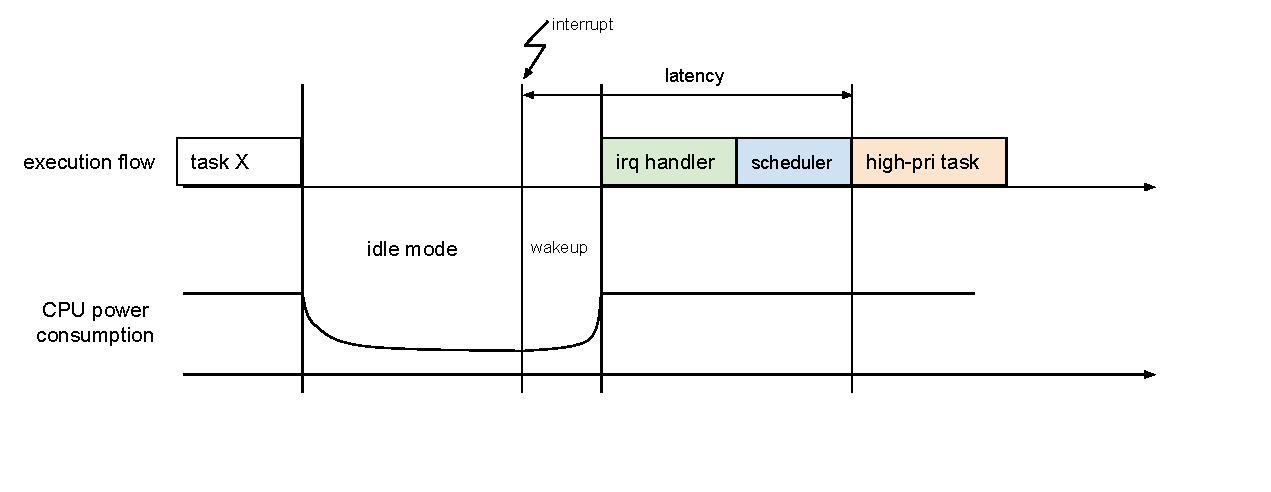
\includegraphics[width=0.8\textwidth]{slides/realtime-linux-hardware/cpuidle_latency}
\end{frame}

\begin{frame}
	\frametitle{Idle States}
	\begin{columns}
		\begin{column}{0.7\textwidth}
			C-States are defined by:
			\begin{itemize}
				\item \code{latency}: The time it takes to wake-up
				\item \code{residency}: Expected sleeping time for which the state can be used
				\item \code{power}: The power consumption in this C-State
			\end{itemize}
			The \code{POLL} state means that the CPU stays in a busy-loop instead of sleeping
		\end{column}
		\begin{column}{0.3\textwidth}
			Idle states, Intel i7-8550U
		    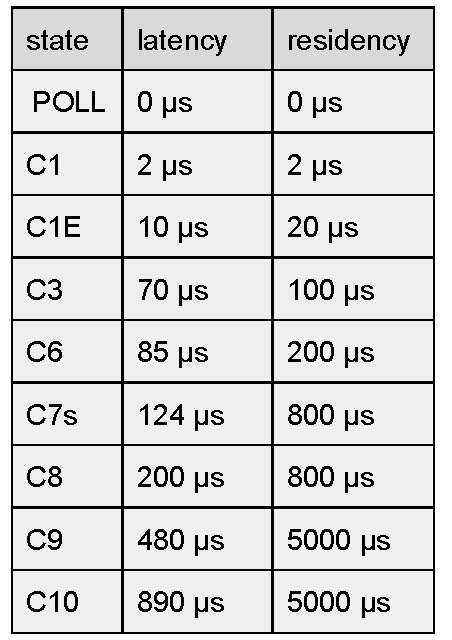
\includegraphics[width=0.8\textwidth]{slides/realtime-linux-hardware/cpu_idle_states_example}
		\end{column}
	\end{columns}
	\vspace{0.5cm}
C-States can be controlled in \code{/sys/devices/system/cpu/cpuX/cpuidle/}
\end{frame}

\begin{frame}
	\frametitle{Limiting the Idle states}
	\begin{itemize}
		\item Limiting the idle states can be done at runtime
			\begin{itemize}
				\item \code{echo 1 > /sys/devices/system/cpu/cpu0/cpuidle/stateX/disable}
			\end{itemize}
		\item C-States can be also limited at boot-time with boot options:
			\begin{itemize}
				\item \code{processor.max_cstates=1}: Limits the deepest sleep state
				\item \code{idle=poll}: Only use polling, never go to sleep
			\end{itemize}
		\item C-States can also be temporarily limited by an application:
			\begin{itemize}
				\item While \code{/dev/cpu_dma_latency} is opened, deep C-States won't be used
				\item Writing \code{0} to this file and maintaining it opened emulates \code{idle=poll}
			\end{itemize}
		\item \textbf{Be careful}, using the \code{POLL} idle state can overheat and destroy your CPU!
	\end{itemize}
\end{frame}

\begin{frame}
	\frametitle{CPU Frequency scaling}
	The CPU frequency can also be dynamically changed through DVFS
	\begin{itemize}
		\item Dynamic Voltage and Frequency Scaling
		\item The frequency can be controlled by the kernel by picking a governor
		\item The governor selects one of the available \textbf{Operating Performance Points}
		\item An \textbf{OPP} defines a frequency and voltage at which a core can run
		\item The \code{performance} governor always uses the highest frequency
		\item The \code{powersave} governor uses the lowest frequency
		\item Other governors can adjust the frequency dynamically
		\item Adjusting the frequency causes non-deterministic execution times
		\item \code{cat /sys/devices/system/cpu/cpu0/cpufreq/scaling_governor}
		\item The governor can also be picked in the Kernel Configuration
	\end{itemize}
\end{frame}

\begin{frame}
	\frametitle{powertop}
	Powertop is a tool to monitor the CPU idle states and frequency usage
	\begin{itemize}
		\item It is designed to optimize the power usage of a system
		\item Useful to undertstand which C-States and OPP are being used
	\end{itemize}
	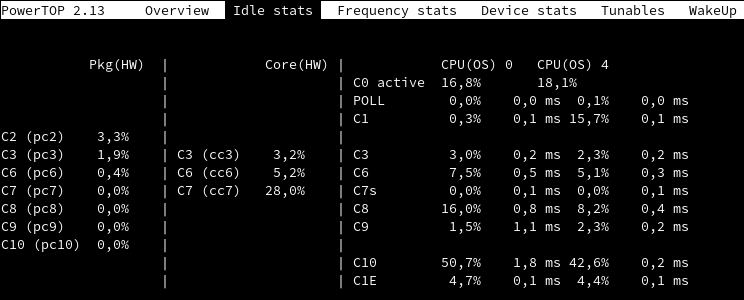
\includegraphics[width=0.8\textwidth]{slides/realtime-linux-hardware/powertop.png}
\end{frame}


